\documentclass[nohyper,justified]{tufte-handout}\usepackage[]{graphicx}\usepackage[]{color}
%% maxwidth is the original width if it is less than linewidth
%% otherwise use linewidth (to make sure the graphics do not exceed the margin)
\makeatletter
\def\maxwidth{ %
  \ifdim\Gin@nat@width>\linewidth
    \linewidth
  \else
    \Gin@nat@width
  \fi
}
\makeatother

\definecolor{fgcolor}{rgb}{0.345, 0.345, 0.345}
\newcommand{\hlnum}[1]{\textcolor[rgb]{0.686,0.059,0.569}{#1}}%
\newcommand{\hlstr}[1]{\textcolor[rgb]{0.192,0.494,0.8}{#1}}%
\newcommand{\hlcom}[1]{\textcolor[rgb]{0.678,0.584,0.686}{\textit{#1}}}%
\newcommand{\hlopt}[1]{\textcolor[rgb]{0,0,0}{#1}}%
\newcommand{\hlstd}[1]{\textcolor[rgb]{0.345,0.345,0.345}{#1}}%
\newcommand{\hlkwa}[1]{\textcolor[rgb]{0.161,0.373,0.58}{\textbf{#1}}}%
\newcommand{\hlkwb}[1]{\textcolor[rgb]{0.69,0.353,0.396}{#1}}%
\newcommand{\hlkwc}[1]{\textcolor[rgb]{0.333,0.667,0.333}{#1}}%
\newcommand{\hlkwd}[1]{\textcolor[rgb]{0.737,0.353,0.396}{\textbf{#1}}}%

\usepackage{framed}
\makeatletter
\newenvironment{kframe}{%
 \def\at@end@of@kframe{}%
 \ifinner\ifhmode%
  \def\at@end@of@kframe{\end{minipage}}%
  \begin{minipage}{\columnwidth}%
 \fi\fi%
 \def\FrameCommand##1{\hskip\@totalleftmargin \hskip-\fboxsep
 \colorbox{shadecolor}{##1}\hskip-\fboxsep
     % There is no \\@totalrightmargin, so:
     \hskip-\linewidth \hskip-\@totalleftmargin \hskip\columnwidth}%
 \MakeFramed {\advance\hsize-\width
   \@totalleftmargin\z@ \linewidth\hsize
   \@setminipage}}%
 {\par\unskip\endMakeFramed%
 \at@end@of@kframe}
\makeatother

\definecolor{shadecolor}{rgb}{.97, .97, .97}
\definecolor{messagecolor}{rgb}{0, 0, 0}
\definecolor{warningcolor}{rgb}{1, 0, 1}
\definecolor{errorcolor}{rgb}{1, 0, 0}
\newenvironment{knitrout}{}{} % an empty environment to be redefined in TeX

\usepackage{alltt}
\usepackage[T1]{fontenc}
\usepackage{url}
\usepackage{mathtools}
%\usepackage{geometry}
%\geometry{verbose,tmargin=2.5cm,bmargin=2.5cm,lmargin=2.5cm,rmargin=2.5cm}
\usepackage{parskip}
\usepackage{enumerate}

%% mess with the fonts
\ifxetex
\usepackage{fontspec}
\defaultfontfeatures{Ligatures=TeX} % To support LaTeX quoting style
%\setromanfont{Times Roman}
\else
\usepackage[T1]{fontenc}
\usepackage[utf8]{inputenc}
%%\fontencoding {T1}
%%\fontfamily {phv}
%%\fontseries {m}
%%\fontshape {n}
%%\fontsize {11pt} {19pt}
%%\linespread {1}
%%\selectfont
\usepackage{sectsty}
\sectionfont{\fontfamily{phv}\fontseries{b}\fontsize{12pt}{20pt}\selectfont}
\subsectionfont{\fontfamily{phv}\fontseries{b}\fontsize{11pt}{20pt}\selectfont}
\subsubsectionfont{\fontfamily{phv}\fontseries{b}\fontsize{11pt}{20pt}\selectfont}
\fi
% For package xtable
\usepackage{booktabs}  % Nice toprules and bottomrules
\heavyrulewidth=1.5pt  % Change the default to heavier lines
\usepackage{longtable} 
\usepackage{tabularx}  % To control the width of the table
%% not used \usepackage{rotating}
%% Not used \usepackage{changepage} % Temporarily change margins -- helpful for wide xtables
%\usepackage[titletoc]{appendix}
%%\usepackage[draft]{pdfpages} % Just inserts a placeholder
\usepackage{enumitem}  % Indents nicely

% this should make caption font bold.
%%\usepackage{caption}
%%\usepackage[margin=.2in,labelfont={rm,bf},textfont={rm},labelsep=period]{caption}
\usepackage{xstring}
\usepackage{etoolbox}
\usepackage{caption}

%%\captionsetup{margin=.2in,labelfont={rm,bf},textfont={rm},font={bf},labelsep=period}

\makeatletter
%\newcommand\formatlabel[1]{%
%    \noexpandarg
%    \IfSubStr{#1}{.}{%
%      \StrBefore{#1}{.}[\firstcaption]%
%      \StrBehind{#1}{.}[\secondcaption]%
%      \textbf{\firstcaption.} \secondcaption}{%
%      #1}%
%      }


%\patchcmd{\@caption}{#3}{\formatlabel{#3}}
\makeatother

%% Url stuff.
\usepackage{url}
\usepackage[unicode=true,
pdfusetitle,
bookmarks=true,
bookmarksnumbered=true,
bookmarksopen=true,
bookmarksopenlevel=2,
breaklinks=true,
pdfborder={0 0 1},
backref=false,
colorlinks=false]{hyperref}

\hypersetup{        
    colorlinks,       % Removing the red boxes
    urlcolor=blue,
    citecolor=black,
    filecolor=black,
    linkcolor=black,
}
\hypersetup{pdfstartview=FitH}

%% xetex only \usepackage{breakurl}
\usepackage{float} % for fig.pos='H'
\usepackage{subfig} % for subfigure
\usepackage{wrapfig}
%%\usepackage{tikz}


% Watermark packages
%\usepackage[firstpage]{draftwatermark}
%\SetWatermarkText{Confidential}
%\SetWatermarkScale{2}
%\SetWatermarkColor[rgb]{0.7,0,0}      % Make text red
%%\usepackage[printwatermark]{xwatermark}
\usepackage{colortbl,xcolor}
%%\newwatermark*[allpages,color=red!50,angle=0,scale=3,xpos=0,ypos=0]{Confidential}

% Both verbatim and comment packages define a comment environment
%usepackage{comment}
\usepackage{verbatim}
% These packages apparently have incompatibilities with others that I use
% You get funky latex error messages if these package refs are placed further up
% Be warned: they may interfere with one or more of the following:
%   url, hyperref, float, subfig, wrapfif, fancyhdr


\makeatletter

%%%%%%%%%%%%%%%%%%%%%%%%%%%%%% LyX specific LaTeX commands.

\title{Homework 2}
\author{Kate Davis}

%%%%%%%%%%%%%%%%%%%%%%%%%%%%%% User specified LaTeX commands.
\renewcommand{\textfraction}{0.05}
\renewcommand{\topfraction}{0.8}
\renewcommand{\bottomfraction}{0.8}
\renewcommand{\floatpagefraction}{0.75}

\usepackage[buttonsize=1em]{animate}

\makeatother

\newcommand{\mms}{M\&Ms\textcopyright}
\newcommand{\dev}[1] {Dev_{\bar{#1}}}
\IfFileExists{upquote.sty}{\usepackage{upquote}}{}
\begin{document}



\maketitle
\section{\mms Data}

\mms \marginnote{http://www.mms.com/} are the colorful candy coated chocolate candies, and are sold with an advertised net weight of $47.9$ grams.

Some curious students acquired $30$ packages of \mms and counted the number of candies in each package, and the total weight of those \mms. After this strenuous exercise, they consumed the evidence.

Using the columns method, compute the Average and Variance of the weight of the candies in the packages, in grams.


The \textbf{mean}\marginnote{The \textbf{Mean} of a data set refers to the arithmetic mean of the values, denoted $\bar{x}$}. The mean is the center that we will use to further examine the ``spread'' of the values.

The mean we use is the arithmetic average, which is calculated by first adding the values of all the observations, then dividing by the number of observations.

\begin{equation*}
\sum\limits_{i=0}^{n} x_i = x_1+x_2+x_3+ \dots +x_{27}+x_{28}+x_{29}+x_{30} 
\end{equation*}

\begin{equation*}
\bar{x}=\frac{\sum\limits_{i=1}^{N} x_i }{N} 
\end{equation*}

\begin{equation*}
Dev_{\bar{x}}=(x_i-\bar{x}) 
\end{equation*}

\begin{equation*}
Dev_{\bar{x}}^2=(x_i-\bar{x})^2 
\end{equation*}

\begin{multline*}
Var(X)=\frac{\sum_{i=1}^{N} Dev_{\bar{x}}^2}{N}=\frac{\sum_{i=1}^{N} (x_i-\bar{x})^2}{N}
\end{multline*}

\begin{equation*}
StdDev(X)=\sqrt{Var(X)} 
\end{equation*}



% latex table generated in R 3.1.2 by xtable 1.7-4 package
% Sun Feb  8 18:52:52 2015
\begin{table}[ht]
\centering
\begin{tabular}{lrll}
  \toprule
Observation & Weight & $\dev{x}$ & ${\dev{x}}^2$ \\ 
  \midrule
$x_{1}$ & 46.22 &              &               \\ 
   \rowcolor[gray]{0.95}$x_{2}$ & 46.72 &              &               \\ 
  $x_{3}$ & 46.94 &              &               \\ 
   \rowcolor[gray]{0.95}$x_{4}$ & 47.61 &              &               \\ 
  $x_{5}$ & 47.67 &              &               \\ 
   \rowcolor[gray]{0.95}$x_{6}$ & 47.70 &              &               \\ 
  $x_{7}$ & 47.98 &              &               \\ 
   \rowcolor[gray]{0.95}$x_{8}$ & 48.28 &              &               \\ 
  $x_{9}$ & 48.33 &              &               \\ 
   \rowcolor[gray]{0.95}$x_{10}$ & 48.45 &              &               \\ 
  $x_{11}$ & 48.49 &              &               \\ 
   \rowcolor[gray]{0.95}$x_{12}$ & 48.72 &              &               \\ 
  $x_{13}$ & 48.74 &              &               \\ 
   \rowcolor[gray]{0.95}$x_{14}$ & 48.95 &              &               \\ 
  $x_{15}$ & 48.98 &              &               \\ 
   \rowcolor[gray]{0.95}$x_{16}$ & 49.16 &              &               \\ 
  $x_{17}$ & 49.40 &              &               \\ 
   \rowcolor[gray]{0.95}$x_{18}$ & 49.69 &              &               \\ 
  $x_{19}$ & 49.79 &              &               \\ 
   \rowcolor[gray]{0.95}$x_{20}$ & 49.80 &              &               \\ 
  $x_{21}$ & 49.80 &              &               \\ 
   \rowcolor[gray]{0.95}$x_{22}$ & 50.01 &              &               \\ 
  $x_{23}$ & 50.23 &              &               \\ 
   \rowcolor[gray]{0.95}$x_{24}$ & 50.40 &              &               \\ 
  $x_{25}$ & 50.43 &              &               \\ 
   \rowcolor[gray]{0.95}$x_{26}$ & 50.97 &              &               \\ 
  $x_{27}$ & 51.53 &              &               \\ 
   \rowcolor[gray]{0.95}$x_{28}$ & 51.68 &              &               \\ 
  $x_{29}$ & 51.71 &              &               \\ 
   \rowcolor[gray]{0.95}$x_{30}$ & 52.06 &              &               \\ 
   \bottomrule
Total & & & \\ 
\rowcolor[gray]{0.95}Total/N & & & \\ 
 & Mean & Zero & Variance \\
\end{tabular}
\caption{Deviations} 
\end{table}



\begin{figure}
\begin{knitrout}
\definecolor{shadecolor}{rgb}{0.969, 0.969, 0.969}\color{fgcolor}

{\centering 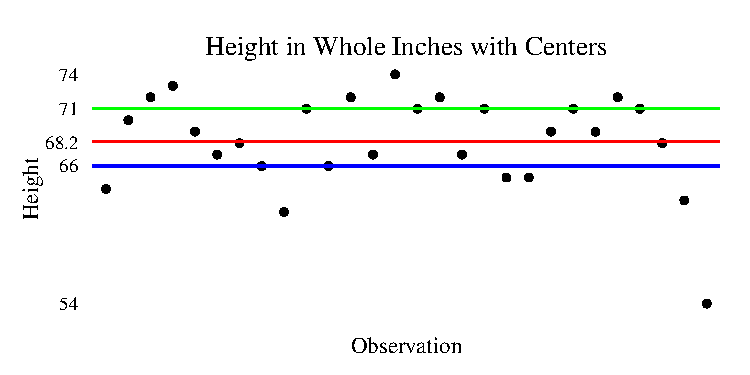
\includegraphics[width=\maxwidth]{figure/graphics-center-chart-1} 

}



\end{knitrout}
\caption{Draw a line at the Mean}
\end{figure}


\end{document}
